\documentclass[12pt]{article}%12-point font
\usepackage[utf8]{inputenc}
\usepackage{amsmath}
\usepackage{mathabx}
\usepackage{graphicx}
\usepackage{siunitx}
\usepackage{commath}
\usepackage{xcolor}
\usepackage{hyperref}
\usepackage{tkz-euclide} %  https://www.mathcha.io/ generates TeX figures 
\usepackage{braket} 
\usepackage{endnotes}
\usepackage{subcaption}
\usepackage{appendix}
\usepackage{float}

\linespread{1.5}%this sets the spacing to 1.5
\usepackage{fullpage}%this sets the margins to 1 inch

\begin{document}


\begin{center}
\begin{LARGE}
\textbf{Supplemental Notes}\\
\end{LARGE}
\end{center}

These notes are provided to acquaint the reader with equations used in the project report. Section (\ref{HK}) derives the Helmholtz-Kirchoff (HK) integral, section (\ref{Rayleigh 1}) uses the HK integral to derive the first Rayleigh integral, section (\ref{Rayleigh 2}) derives the second Rayleigh integral, and sections (\ref{Fraunhofer}) and (\ref{Fresnel}) respectively take the Fraunhofer and Fresnel limits.

\section{Derivation of the HK integral}\label{HK}

The HK integral is the solution $p(\boldsymbol r)$ to the inhomogenous Helmholtz equation,

\begin{equation}\label{wave eq}
\nabla^2 p(\boldsymbol r) + k^2 p(\boldsymbol r) = -f(\boldsymbol r),  
\end{equation}

\noindent where the inhomogenity is described by the distribution function $f(\boldsymbol r)$. To derive the HK integral, first recall that the free space Green's function $g (\boldsymbol r| \boldsymbol r_0)$ solves 

\begin{equation}\label{definition}
\nabla^2 g (\boldsymbol r | \boldsymbol r_0) + k^2 g (\boldsymbol r | \boldsymbol r_0) = -\delta (\boldsymbol r - \boldsymbol r_0).
\end{equation}

\noindent Also suppose $\chi(\boldsymbol r)$ is solution to the homogeneous Helmholtz equation:
\begin{equation}\label{homo}
    \nabla^2 \chi + k^2 \chi = 0.
\end{equation}


\noindent Since the general solution is the sum of the inhomogeneous and homogeneous solutions,  $G(\boldsymbol r_0| \boldsymbol r) = g(\boldsymbol r_0| \boldsymbol r) + \chi (\boldsymbol r)$ is the general solution to equation (\ref{definition}). That is,

\begin{equation}\label{forbigG}
\nabla^2 G (\boldsymbol r | \boldsymbol r_0) + k^2 G (\boldsymbol r | \boldsymbol r_0) = -\delta (\boldsymbol r - \boldsymbol r_0).
\end{equation}

\noindent Next, equation (\ref{forbigG}) is multiplied by $p(\boldsymbol r)$ and subtracted from the product of $G$ and equation (\ref{wave eq}):

\begin{align}\label{transform}
    G(\boldsymbol r| \boldsymbol r_0) \nabla^2 p(\boldsymbol r) - p(\boldsymbol r) \nabla^2 G(\boldsymbol r| \boldsymbol r_0) = -f(\boldsymbol r) G(\boldsymbol r| \boldsymbol r_0) + p(\boldsymbol r) \delta (\boldsymbol r - \boldsymbol r_0)
\end{align}

\noindent Now switching the location of the source from $\boldsymbol r_0$ to $\boldsymbol r$, $f(\boldsymbol r_0) \mapsto f(\boldsymbol r)$, so equation (\ref{transform}) becomes

\begin{align}\label{transform1}
    G(\boldsymbol r| \boldsymbol r_0) \nabla^2 p(\boldsymbol r) - p(\boldsymbol r) \nabla^2 G(\boldsymbol r| \boldsymbol r_0) = -f(\boldsymbol r_0) G(\boldsymbol r| \boldsymbol r_0) + p(\boldsymbol r) \delta (\boldsymbol r - \boldsymbol r_0)
\end{align}

\noindent Further, since $G$ satisfies reciprocity, $G(\boldsymbol r | \boldsymbol r_0) = G(\boldsymbol r_0 | \boldsymbol r)$. Recall also that $\delta(\boldsymbol r - \boldsymbol r_0) = \delta(\boldsymbol r_0 - \boldsymbol r)$. Making these transformations to equation (\ref{transform1}) yields

\begin{align}\label{new}
    G(\boldsymbol r_0| \boldsymbol r) \nabla^2 p(\boldsymbol r_0) - p(\boldsymbol r_0) \nabla^2 G(\boldsymbol r_0| \boldsymbol r) = -f(\boldsymbol r_0) G(\boldsymbol r_0| \boldsymbol r) + p(\boldsymbol r_0) \delta (\boldsymbol r_0 - \boldsymbol r)
\end{align}


\noindent Integrating (\ref{new}) in the `$_0$' coordinates,

\begin{align*}
    \iiint \big\lbrace G(\boldsymbol r_0| \boldsymbol r) \nabla^2 p(\boldsymbol r_0) -& p(\boldsymbol r_0) \nabla^2 G(\boldsymbol r_0| \boldsymbol r) \big\rbrace dv_0 = \\ &\iiint \big\lbrace -f(\boldsymbol r_0) G(\boldsymbol r_0| \boldsymbol r) + p(\boldsymbol r_0) \delta (\boldsymbol r_0 - \boldsymbol r)\big\rbrace dv_0
\end{align*}

\noindent Applying the sifting property of the delta function on the right-hand-side, writing $G(\boldsymbol r_0| \boldsymbol r) \nabla^2 p(\boldsymbol r_0) - p(\boldsymbol r_0) \nabla^2 G(\boldsymbol r_0| \boldsymbol r) = \boldsymbol \nabla_0 \cdot (G(\boldsymbol r_0| \boldsymbol r) \boldsymbol\nabla p(\boldsymbol r_0) - p(\boldsymbol r_0) \boldsymbol\nabla  G(\boldsymbol r_0| \boldsymbol r))$, and solving for $p(\boldsymbol r_0)$,

\begin{align*}
    p(\boldsymbol r) &= \iiint f(\boldsymbol r_0) G(\boldsymbol r_0| \boldsymbol r) dv_0 +  \iiint \boldsymbol \nabla_0 \cdot \big\lbrace G(\boldsymbol r_0| \boldsymbol r) \boldsymbol\nabla p(\boldsymbol r_0) - p(\boldsymbol r_0) \boldsymbol\nabla  G(\boldsymbol r_0| \boldsymbol r)\big\rbrace dv_0
\end{align*}

\noindent Utilizing the divergence theorem on the left-hand-side, writing the gradients as $\pd{}{n_0}$, and utilizing $G(\boldsymbol r_0|\boldsymbol r) = G(\boldsymbol r|\boldsymbol r_0)$ (mainly to match Dr. Hamilton's notes), 

\begin{align*}
    p(\boldsymbol r) &= \iiint f(\boldsymbol r_0) G(\boldsymbol r_0| \boldsymbol r) dv_0 +  \oiint \big\lbrace G(\boldsymbol r| \boldsymbol r_0) \pd{}{n_0} p(\boldsymbol r_0) - p(\boldsymbol r_0) \pd{}{n_0}  G(\boldsymbol r| \boldsymbol r_0) \big\rbrace dS_0\tag{HK integral}
\end{align*}

\noindent This is the Helmholtz-Kirchoff integral, which is used in section (\ref{Rayleigh 1}) to derive the Rayleigh integral. 

\section{Derivation of the first Rayleigh integral}\label{Rayleigh 1}

\begin{figure}%
    \centering
\tikzset{every picture/.style={line width=0.75pt}} %set default line width to 0.75pt        

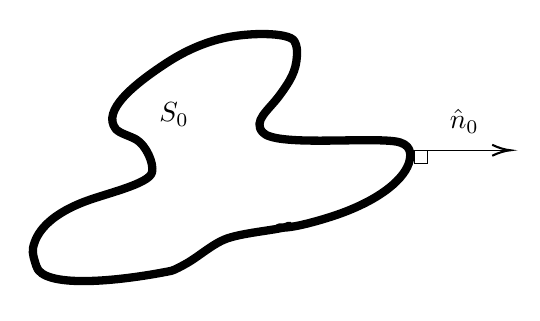
\begin{tikzpicture}[x=0.6pt,y=0.6pt,yscale=-1,xscale=1]
%uncomment if require: \path (0,300); %set diagram left start at 0, and has height of 300

%Shape: Free Drawing [id:dp6784340293297795] 
\draw  [color={rgb, 255:orange, 0; orange, 0; cyan, 0 }  ][line width=3] [line join = round][line cap = round] (368.71,162.49) .. controls (376.03,163.55) and (396.08,157.42) .. (403.41,154.89) .. controls (430.3,145.63) and (445.27,132.48) .. (447.38,121.87) .. controls (448.13,118.08) and (448.49,111.8) .. (437.98,110.56) .. controls (418.09,108.23) and (366.34,113.74) .. (358.84,105.22) .. controls (352.73,98.28) and (362.39,91.89) .. (368.72,83.33) .. controls (375.87,73.65) and (378.88,68.28) .. (379.47,59.26) .. controls (379.68,56.14) and (379.58,53.02) .. (377.92,50.24) .. controls (374.6,44.67) and (348.28,44.8) .. (331.82,49.3) .. controls (318.48,52.94) and (308.22,58.64) .. (300.75,63.54) .. controls (281.2,76.34) and (261.75,92.24) .. (270.32,103.11) .. controls (272.43,105.78) and (278.76,107.28) .. (282.6,109.48) .. controls (288.56,112.9) and (293.46,123.79) .. (292.21,129.23) .. controls (290.56,136.4) and (264.04,142.03) .. (250.63,147.3) .. controls (229.47,155.62) and (222.28,166.15) .. (220.58,174.69) .. controls (219.81,178.57) and (221.49,182.08) .. (222.48,185.68) .. controls (226.2,199.34) and (270.41,195.28) .. (303.69,188.64) .. controls (305.68,188.24) and (311.38,185.02) .. (311.72,184.83) .. controls (319.98,180.48) and (328.59,172.17) .. (337.56,169.07) .. controls (348.75,165.22) and (370.03,163.93) .. (374.74,161.45) ;
%Straight Lines [id:da14503798684826585] 
\draw    (450,116) -- (506,116) ;
\draw [shift={(508,116)}, rotate = 180] [color={rgb, 255:orange, 0; orange, 0; cyan, 0 }  ][line width=0.75]    (10.93,-3.29) .. controls (6.95,-1.4) and (3.31,-0.3) .. (0,0) .. controls (3.31,0.3) and (6.95,1.4) .. (10.93,3.29)   ;
%Shape: Rectangle [id:dp16851011786982473] 
\draw   (450,116) -- (458,116) -- (458,124) -- (450,124) -- cycle ;

% Text Node
\draw (295,86) node [anchor=north west][inner sep=0.75pt]   [align=left] {$\displaystyle S_{0}$};
% Text Node
\draw (470,90) node [anchor=north west][inner sep=0.75pt]   [align=left] {$\displaystyle \hat{n}_{0}$};
\end{tikzpicture}
  \caption{Closed surface $S_0$ subjected to a source condition at the surface and containing no sources in the enclosed volume.}%
    \label{potato}
\end{figure} 

Consider a closed surface $S_0$ that is subjected to a velocity source condition on the boundary and contains no sources within the enclosed volume, as illustrated in figure (\ref{potato}). Since there are no sources in the enclosed volume, the volume integral term of the (HK integral) vanishes, leaving

\begin{align}\label{new HK}
    p(\boldsymbol r) &= \oiint \big\lbrace \color{cyan}G(\boldsymbol r| \boldsymbol r_0) \color{orange}\pd{}{n_0} p(\boldsymbol r) \color{black}- \underline{ p(\boldsymbol r) \pd{}{n_0}  G(\boldsymbol r| \boldsymbol r_0)} \big\rbrace dS_0
\end{align}

\noindent The boundary of interest is a rigid plane at $z=0$, portions of which vibrate in the $z$-direction, as shown in figure (\ref{specific potato}).  A velocity source condition is defined:

\begin{figure}%
    \centering
    


\tikzset{every picture/.style={line width=0.75pt}} %set default line width to 0.75pt        

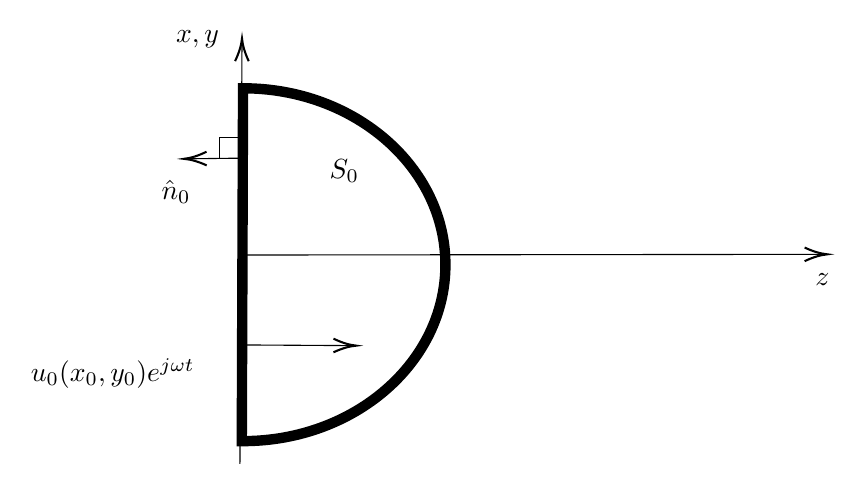
\begin{tikzpicture}[x=0.75pt,y=0.75pt,yscale=-1,xscale=1]
%uncomment if require: \path (0,238); %set diagram left start at 0, and has height of 238

%Straight Lines [id:da7769318630531843] 
\draw    (200.5,119.67) -- (481,119.34) ;
\draw [shift={(483,119.33)}, rotate = 179.93] [color={rgb, 255:red, 0; green, 0; blue, 0 }  ][line width=0.75]    (10.93,-3.29) .. controls (6.95,-1.4) and (3.31,-0.3) .. (0,0) .. controls (3.31,0.3) and (6.95,1.4) .. (10.93,3.29)   ;
%Straight Lines [id:da2339344712004492] 
\draw    (200,220.33) -- (200.99,17.33) ;
\draw [shift={(201,15.33)}, rotate = 90.28] [color={rgb, 255:red, 0; green, 0; blue, 0 }  ][line width=0.75]    (10.93,-3.29) .. controls (6.95,-1.4) and (3.31,-0.3) .. (0,0) .. controls (3.31,0.3) and (6.95,1.4) .. (10.93,3.29)   ;
%Shape: Chord [id:dp09338432502464555] 
\draw  [line width=3.75]  (200.89,209.33) .. controls (201.09,209.33) and (201.3,209.33) .. (201.5,209.33) .. controls (255.35,209.33) and (299,171.28) .. (299,124.33) .. controls (299,77.39) and (255.35,39.33) .. (201.5,39.33) -- cycle ;
%Straight Lines [id:da20362955787977555] 
\draw    (200,73) -- (175,73.31) ;
\draw [shift={(173,73.33)}, rotate = 359.29] [color={rgb, 255:red, 0; green, 0; blue, 0 }  ][line width=0.75]    (10.93,-3.29) .. controls (6.95,-1.4) and (3.31,-0.3) .. (0,0) .. controls (3.31,0.3) and (6.95,1.4) .. (10.93,3.29)   ;
%Straight Lines [id:da22600481599024014] 
\draw    (203,163) -- (254,163.32) ;
\draw [shift={(256,163.33)}, rotate = 180.36] [color={rgb, 255:red, 0; green, 0; blue, 0 }  ][line width=0.75]    (10.93,-3.29) .. controls (6.95,-1.4) and (3.31,-0.3) .. (0,0) .. controls (3.31,0.3) and (6.95,1.4) .. (10.93,3.29)   ;
%Shape: Square [id:dp5200120435388684] 
\draw   (190,63) -- (200,63) -- (200,73) -- (190,73) -- cycle ;

% Text Node
\draw (476,127.4) node [anchor=north west][inner sep=0.75pt]    {$z$};
% Text Node
\draw (168,10.4) node [anchor=north west][inner sep=0.75pt]    {$x,y$};
% Text Node
\draw (242,72.4) node [anchor=north west][inner sep=0.75pt]    {$S_{0}$};
% Text Node
\draw (161,82.4) node [anchor=north west][inner sep=0.75pt]    {$\hat{n}_{0}$};
% Text Node
\draw (98,168.4) node [anchor=north west][inner sep=0.75pt]    {$u_{0}( x_{0} ,y_{0}) e^{j\omega t}$};


\end{tikzpicture}

    \caption{Specialization of figure (\ref{potato}) to a vibrating velocity source at $z=0$. Note that the unit normal vector $\hat n_0$ points in the opposite direction as the $z$-axis.}%
    \label{specific potato}
\end{figure}   
    

\begin{align}\label{velocity source condition}
u(x,y,z=0,t) = u_0 (x_0,y_0) e^{-i\omega t}    
\end{align}

\noindent Equation (\ref{velocity source condition}) can be incorporated into the \color{orange}second factor \color{black} of equation (\ref{new HK}) using the momentum equation, $\pd{p(\boldsymbol r_0)}{n_0} =-\pd{p(x_0,y_0)}{z_0}= -\rho_0 \pd{u(x,y,z=0,t)}{t}$, which simplifies to

\begin{align*}
    \color{orange}\pd{p(x_0,y_0)}{z_0} \color{black}&= \rho_0 \pd{u_0(x_0,y_0)e^{-i\omega t}}{t}\\
    &= \color{orange} -i\omega \rho_0 u_0(x_0, y_0) \tag{\color{orange} second factor\color{black}}
\end{align*}


\noindent Next, it is desirable to choose a Green's function that makes the \underline{underlined term} in equation (\ref{new HK}) vanish (i.e., $\pd{G}{n_0} = 0$ on $S_0$). Denoting 
$$g_\pm = \frac{e^{ikR_\pm}}{4\pi R_\pm},$$ 
\noindent where 

$$R_\pm = \sqrt{(x-x_0)^2 + (y-y_0)^2 + (z\mp z_0)^2},$$ 

\noindent one such choice is 

\begin{align}\label{Green's function for derivation}
G(\boldsymbol r | \boldsymbol r_0) &= g_+(\boldsymbol r | \boldsymbol r_0) + g_-(\boldsymbol r | \boldsymbol r_0)   
\end{align}
 
\noindent Upon this choice of the Green's function, and setting $z_0 = 0$ because the source is in the $z=0$ plane, the \color{cyan} first factor \color{black} of equation (\ref{new HK}) becomes

\begin{align*}
\color{cyan} G(\boldsymbol r|\boldsymbol r_0) \bigg\rvert_{z_0=0} \color{black}  &=2g(\boldsymbol r|\boldsymbol r_0) \\ 
&= \frac{e^{ikR}}{4\pi R} + \frac{e^{ikR}}{4\pi R}\\
&= \color{cyan} \frac{e^{ikR}}{2\pi R} \tag{\color{cyan} first factor} 
\end{align*}

\color{black}

\noindent where \color{cyan}  $R = \sqrt{(x-x_0)^2 + (y-y_0)^2 + z^2}$\color{black}. Substituting the (\color{orange}second factor\color{black})   and the (\color{cyan}first factor\color{black})  into equation (\ref{new HK}) gives

\begin{align*}
p(\boldsymbol{r}) &=  \oiint \color{orange}(-i\omega \rho_0 u_0(x_0, y_0)) \color{cyan} \frac{e^{ikR}}{2\pi R} \color{black} \dif S  \\
&= -i\frac{\rho_0 c_0 k}{2\pi} \oiint \frac{u_0(x_0, y_0) e^{ikR}}{R} \color{black} \dif S \tag{first Rayleigh integral}
\end{align*}

\noindent The (first Rayleigh integral) matches equation (1) in Terzi et al. upon notation of the amplitude of the normal component of vibration velocity $u_0(x_0, y_0) \equiv V$. 

\begin{equation}
p = -i \frac{\rho_0 c_0 k}{2\pi} \oiint \frac{V e^{ikR}}{R}\dif S 
\end{equation}




\section{Derivation of the second Rayleigh integral}\label{Rayleigh 2}

\begin{figure}%
    \centering
    

\tikzset{every picture/.style={line width=0.75pt}} %set default line width to 0.75pt        

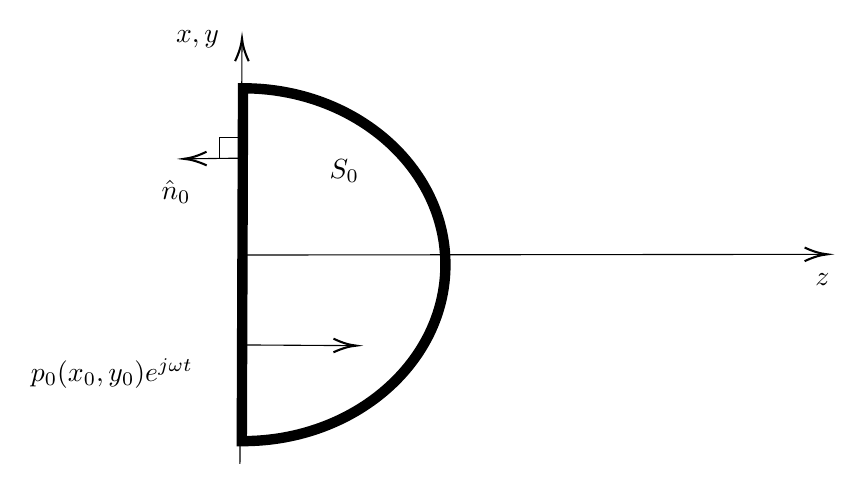
\begin{tikzpicture}[x=0.75pt,y=0.75pt,yscale=-1,xscale=1]
%uncomment if require: \path (0,238); %set diagram left start at 0, and has height of 238

%Straight Lines [id:da7769318630531843] 
\draw    (200.5,119.67) -- (481,119.34) ;
\draw [shift={(483,119.33)}, rotate = 179.93] [color={rgb, 255:red, 0; green, 0; blue, 0 }  ][line width=0.75]    (10.93,-3.29) .. controls (6.95,-1.4) and (3.31,-0.3) .. (0,0) .. controls (3.31,0.3) and (6.95,1.4) .. (10.93,3.29)   ;
%Straight Lines [id:da2339344712004492] 
\draw    (200,220.33) -- (200.99,17.33) ;
\draw [shift={(201,15.33)}, rotate = 90.28] [color={rgb, 255:red, 0; green, 0; blue, 0 }  ][line width=0.75]    (10.93,-3.29) .. controls (6.95,-1.4) and (3.31,-0.3) .. (0,0) .. controls (3.31,0.3) and (6.95,1.4) .. (10.93,3.29)   ;
%Shape: Chord [id:dp09338432502464555] 
\draw  [line width=3.75]  (200.89,209.33) .. controls (201.09,209.33) and (201.3,209.33) .. (201.5,209.33) .. controls (255.35,209.33) and (299,171.28) .. (299,124.33) .. controls (299,77.39) and (255.35,39.33) .. (201.5,39.33) -- cycle ;
%Straight Lines [id:da20362955787977555] 
\draw    (200,73) -- (175,73.31) ;
\draw [shift={(173,73.33)}, rotate = 359.29] [color={rgb, 255:red, 0; green, 0; blue, 0 }  ][line width=0.75]    (10.93,-3.29) .. controls (6.95,-1.4) and (3.31,-0.3) .. (0,0) .. controls (3.31,0.3) and (6.95,1.4) .. (10.93,3.29)   ;
%Straight Lines [id:da22600481599024014] 
\draw    (203,163) -- (254,163.32) ;
\draw [shift={(256,163.33)}, rotate = 180.36] [color={rgb, 255:red, 0; green, 0; blue, 0 }  ][line width=0.75]    (10.93,-3.29) .. controls (6.95,-1.4) and (3.31,-0.3) .. (0,0) .. controls (3.31,0.3) and (6.95,1.4) .. (10.93,3.29)   ;
%Shape: Square [id:dp5200120435388684] 
\draw   (190,63) -- (200,63) -- (200,73) -- (190,73) -- cycle ;

% Text Node
\draw (476,127.4) node [anchor=north west][inner sep=0.75pt]    {$z$};
% Text Node
\draw (168,10.4) node [anchor=north west][inner sep=0.75pt]    {$x,y$};
% Text Node
\draw (242,72.4) node [anchor=north west][inner sep=0.75pt]    {$S_{0}$};
% Text Node
\draw (161,82.4) node [anchor=north west][inner sep=0.75pt]    {$\hat{n}_{0}$};
% Text Node
\draw (98,168.4) node [anchor=north west][inner sep=0.75pt]    {$p_{0}( x_{0} ,y_{0}) e^{j\omega t}$};


\end{tikzpicture}
    \caption{Specialization of figure (\ref{potato}) to a vibrating rigid pressure source at $z=0$.}%
    \label{specific potato 2}
\end{figure}   
    
Consider a closed surface $S_0$ that is subjected to a pressure source condition on the boundary and contains no sources within the enclosed volume, as illustrated in figure (\ref{specific potato 2}). Since there are no sources in the enclosed volume, the volume integral term of the (HK integral) vanishes, leaving

\begin{align}\label{new HK 2}
    p(\boldsymbol r) &= \oiint \big\lbrace \underline{G(\boldsymbol r| \boldsymbol r_0) \pd{}{n_0} p(\boldsymbol r)} -  \color{cyan}p(\boldsymbol r) \color{orange}\pd{}{n_0}  G(\boldsymbol r| \boldsymbol r_0)\color{black} \big\rbrace dS_0
\end{align}

\noindent The boundary of interest is a pressure source at $z=0$ that vibrates in the $z$-direction. A pressure source condition is defined:

\begin{align}\label{pressure source condition}
p(x,y,z=0,t) = p_0 (x_0,y_0) e^{-i\omega t}    
\end{align}

\noindent Equation (\ref{pressure source condition}) is incorporated into the \color{cyan}first factor \color{black} of equation (\ref{new HK 2}) by simply removing the $e^{-i\omega t}$ time dependence.
 
Next, it is desirable to choose a Green's function that makes the \underline{underlined term} in equation (\ref{new HK 2}) vanish (i.e., $G = 0$ on $S_0$). Denoting as before
$$g_\pm = \frac{e^{ikR_\pm}}{4\pi R_\pm},$$ 
\noindent where 

$$R_\pm = \sqrt{(x-x_0)^2 + (y-y_0)^2 + (z\mp z_0)^2},$$ 

\noindent one such choice is 

\begin{align}\label{Green's function for derivation}
G(\boldsymbol r | \boldsymbol r_0) &= g_+(\boldsymbol r | \boldsymbol r_0) - g_-(\boldsymbol r | \boldsymbol r_0)   
\end{align}
 
\noindent Upon this choice of the Green's function, and setting $z_0 = 0$ because the source is in the $z=0$ plane, $G(\boldsymbol r|\boldsymbol r_0)$ in the underlined term vanishes indeed:

\begin{align*}
G(\boldsymbol r|\boldsymbol r_0) \bigg\rvert_{z_0=0} &=  \frac{e^{ikR}}{4\pi R} - \frac{e^{ikR}}{4\pi R} =0
\end{align*}

\noindent where $R = \sqrt{(x-x_0)^2 + (y-y_0)^2 + z^2}$. 


Meanwhile, the \color{orange} second factor \color{black} of equation (\ref{new HK}) becomes

\begin{align*}
\color{orange} \frac{\partial}{\partial n_0} G(\boldsymbol r|\boldsymbol r_0)\bigg\rvert_{z_0=0}\color{black}&= -\frac{\partial}{\partial z_0} \Bigg\lbrack\frac{e^{ik\sqrt{(x-x_0)^2+(y-y_0)^2 +(z-z_0)^2}}}{\sqrt{(x-x_0)^2+(y-y_0)^2 +(z-z_0)^2}}\\  
&\text{\space \space \space \space \space \space \space \space \space \space \space \space }- \frac{e^{ik\sqrt{(x-x_0)^2+(y-y_0)^2 +(z-z_0)^2}}}{\sqrt{(x-x_0)^2+(y-y_0)^2 +(z-z_0)^2}}\Bigg\rbrack\Bigg\rvert_{z_0=0} \\ 
&=  -\frac{1}{2\pi}\del{ik e^{ikR}z R^{-2} + e^{ikR} z R^{-3} }\\
&= \color{orange} \frac{z}{2\pi}\frac{e^{ikR}}{R}\del{-\frac{ik}{R} + \frac{1}{R^2}} \tag{\color{orange} second factor\color{black}}
\end{align*}



\noindent where again \color{orange}  $R = \sqrt{(x-x_0)^2 + (y-y_0)^2 + z^2}$\color{black}. Substituting the (\color{orange}second factor\color{black})   and the (\color{cyan}first factor\color{black})  into equation (\ref{new HK}) gives

\begin{align*}
p(\boldsymbol{r}) &=  \oiint \color{cyan} p_0 (x_0,y_0) \color{black} \color{orange} \frac{z}{2\pi}\frac{e^{ikR}}{R}\del{-\frac{ik}{R} + \frac{1}{R^2}}\color{black}  \dif S_0  \\
&= \frac{z}{2\pi} \oiint p_0(x_0, y_0)  \del{-\frac{ik}{R} + \frac{1}{R^2}}\frac{e^{ikR}}{R} \dif S_0 \tag{second Rayleigh integral}
\end{align*}

\noindent The (second Rayleigh integral) matches equation (2) in Terzi et al. upon translation from $\boldsymbol r_0 = (x_0,y_0,z_0)$ to $\boldsymbol r_1 = (x_1,y_1,z_0-z_1)$ and using $p(\boldsymbol r_1)$ instead of $p_0(x_0,y_0) = p(\boldsymbol r_0)$.



\section{Fraunhofer limit}\label{Fraunhofer}

\section{Fresnel limit}\label{Fresnel}










\begin{thebibliography}{99}

\iffalse
\bibitem{ref1}
Terzi, M. E., Tsysar, S. A., Yuldashev, P. V., Karzova, M. M., and Sapozhnikov, O. A. \href{https://doi.org/10.3103/S0027134916050180}{Generation of a vortex ultrasonic beam with a phase plate with an angular dependence of the thickness}. \textit{Moscow University Physics Bulletin}. \textbf{72}, 61–67 (2017).


\bibitem{ref2}
Melde, K., Mark, A. G., Qiu, T., and Fischer, P. \href{https://doi.org/10.1038/nature19755}{Holograms for acoustics}. \textit{Nature}. \textbf{537}, 518–522 (2016).

\bibitem{ref3} 
Sallam, A., Meesala, V.C., Hajj, M.R., et al. \href{https://doi.org/10.1063/5.0065489}{Holographic mirrors for spatial ultrasound modulation in contactless acoustic energy transfer systems}.  \textit{Applied Physics Letters}. \textbf{119}, 144101 (2021).

\bibitem{ref4} 
Parker, S. \href{https://hdl.handle.net/2152/87049}{Physical limitations and practical considerations for the creation of acoustic holograms}. M.S. Thesis, The University of Texas at Austin. (2020).

\bibitem{ref5} 
Sapozhnikov, O.A., Tsysar, S.A., et al. \href{https://doi.org/10.1121/1.4928396}{Acoustic holography as a metrological tool for characterizing medical ultrasound sources and fields}. \textit{The Journal of the Acoustical Society of America} \textbf{138}, 1515 (2015). 
\fi

\end{thebibliography}
\end{document}


